% begin module exponential-function-properties
\begin{frame}
\begin{columns}[t]
\column{.3\textwidth}
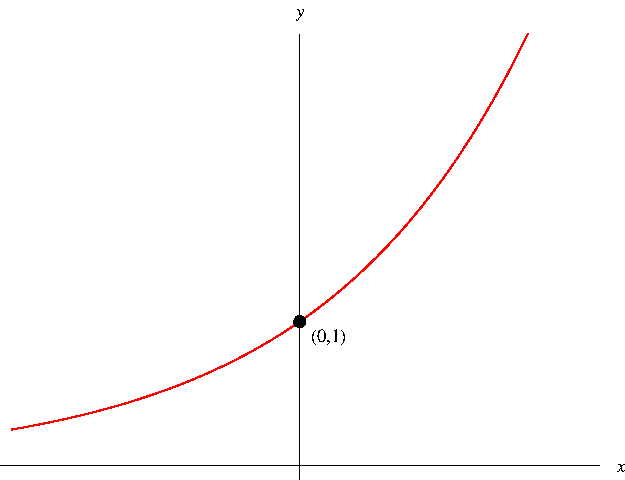
\includegraphics[height=3cm]{exponential-functions/pictures/07-02-exptypesa.pdf}%

$y = a^x, a > 1$
\begin{itemize}
\item<2->  Increasing.
\item<3->  Passes through $(0,1)$.
\item<4->  $\lim_{x \rightarrow \infty} a^x = \infty$.
\item<5->  $\lim_{x \rightarrow -\infty} a^x = 0$.
\end{itemize}
\column{.35\textwidth}
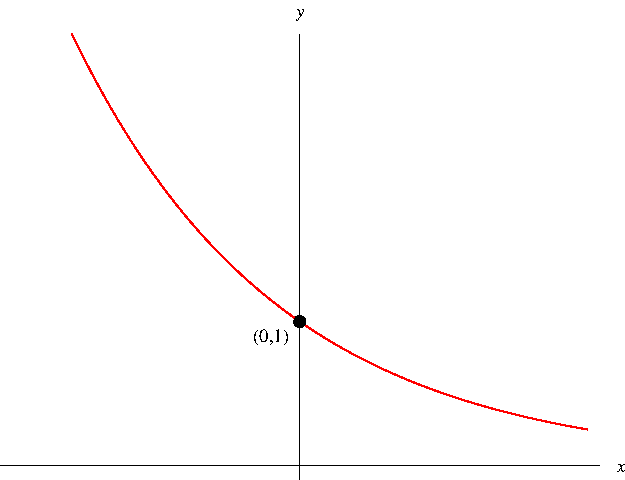
\includegraphics[height=3cm]{exponential-functions/pictures/07-02-exptypesb.pdf}%

$y = a^x, 0 < a < 1$
\begin{itemize}
\item<6->  Decreasing.
\item<7->  Passes through $(0,1)$.
\item<8->  $\left(\frac{1}{a}\right)^x = a^{-x}$.
\item<9->  Reflection of $y = \left(\frac{1}{a}\right)^x$ in the $y$-axis.
\item<10->  $\lim_{x \rightarrow \infty} a^x = 0$.
\item<11->  $\lim_{x \rightarrow -\infty} a^x = \infty$.
\end{itemize}
\column{.3\textwidth}
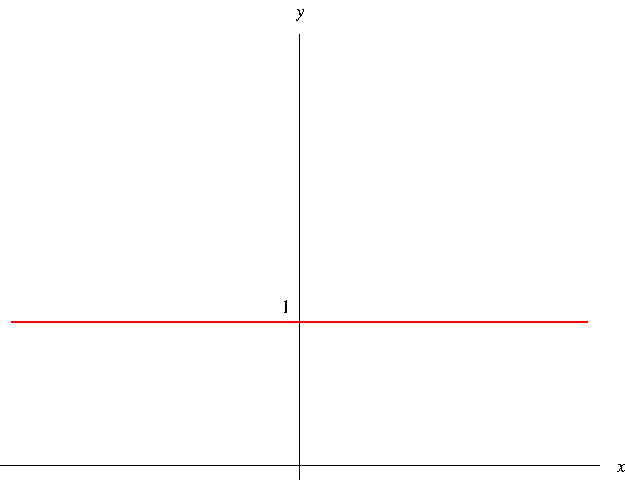
\includegraphics[height=3cm]{exponential-functions/pictures/07-02-exptypesc.pdf}%

$y = a^x, a = 1$
\begin{itemize}
\item<12->  Horizontal.
\end{itemize}
\end{columns}
\end{frame}


\begin{frame}
\begin{theorem}[Properties of Exponential Functions]
If $a > 0$ and $a \neq 1$, then $f(x) = a^x$ is a continuous function with domain $\mathbb{R}$ and range $(0,\infty )$.  In particular, $a^x > 0$ for all $x$.  If $0 < a < 1$, then $f(x) = a^x$ is a decreasing function; if $a > 1$, then $f(x) = a^x$ is an increasing function.  If $a, b > 0$ and $x, y \in\mathbb{R}$, then
\begin{enumerate}
\item  $a^{x+y} = a^xa^y$
\item  $a^{x-y} = \frac{a^x}{a^y}$
\item  $(a^x)^y = a^{xy}$
\item  $(ab)^x = a^xb^x$
\item  If $a > 1$, then $\lim_{x\rightarrow \infty} a^x = \infty$ and $\lim_{x\rightarrow -\infty} a^x = 0$.
\item  If $0 < a < 1$, then $\lim_{x\rightarrow \infty} a^x = 0$ and $\lim_{x\rightarrow -\infty} a^x = \infty$.
\end{enumerate}
In particular, if $a \neq 1$, then the $x$-axis is a horizontal asymptote for $y = a^x$. 
\end{theorem}
\end{frame}
% end module exponential-function-properties
